\documentclass[12pt]{article}
\usepackage{graphicx} % Required for inserting images

\title{Learning ML/DL}
\author{Benjamin Li}
\date{2025}
\usepackage{setspace}
\usepackage{amsmath}
\usepackage{color,soul}
\usepackage{amsmath}
\usepackage{nicefrac}
\usepackage{amsfonts}
\usepackage{amsthm}
% \usepackage{url}
\usepackage{float} % Add this line near the top with other \usepackage statements

% \usepackage{breakurl}
\usepackage{hyperref}
\usepackage[margin=1in]{geometry}
\renewcommand{\baselinestretch}{1.3} 

% nicefrac package? 
% make macro/keybinds to create the matrices/other things

\newcommand{\lnn}[1]{%
  \ln\left(#1\right)%
}

\newcommand{\logp}[1]{%
  \log\left(#1\right)%
}

\newcommand{\sigp}[1]{%
  \sigma\left(#1\right)%
}


\begin{document}

\maketitle

\section{Introduction}

This document serves as an aggregation of my progress towards gaining a more fundamental understanding of how many modern ML/DL models work. To understand it, an introductory background in linear algebra (matrix operations), calculus (derivatives), and probability is assumed. Corresponding code implementations will be made available in the future, and some helpful references are included for each section. This document is also a bit text-dense so I hope to add some of my diagrams/drawings later. 


\section{Multilayer Perceptron (Fully-Connected Neural Network)}
\subsection{Overview and Network Initialization}

First, let's look at a specific example. Let's say we have 10 soccer players (and two pieces of info - \textbf{features} - about their record number of consecutive juggles and weight in kilograms) and we want to determine if they're going to be drafted to a soccer team. Mathematically, we are given a batched input $x$ of dimensions $(b, f)$, where $b$ is the number of entries and $f$ is the number of features. In our case, let’s say it's $(10, 2)$. 

\[x=\begin{bmatrix}
50 & 75 \\
80 & 68 \\
100 & 80 \\
\vdots & \vdots \\
40 & 60
\end{bmatrix}, y=\begin{bmatrix}
0 \\
1 \\
1 \\
\vdots \\
0
\end{bmatrix}\]


We are trying to predict a vector $y$ of dimensions $(10, 1)$ where 1 indicates that a player is drafted and 0 indicates they are not drafted. 

To do this, we construct a \textbf{fully-connected neural network}. This architecture consists of multiple \textbf{layers}, and within each layer multiple \textbf{neurons}. Thus, before constructing the network we initialize an array $n = [2, 3, 4, 5, 1]$ in which each index represents the number of neurons for the corresponding layer. Notably, the index 0 represents the INPUT dimension, and index 4 is the OUTPUT dimension (must be 1 since we’re trying to predict one outcome). Finally, randomly initialize a list of weights and biases (more details later). At a high level, training neural networks involves two steps: \textbf{feedforward} and \textbf{backpropagation}, and these are the next two sections. 


\subsection{Feedforward Process}

Each layer $i$ calculates the following:
\[A_i = \sigma(W_i * A_{i-1} + B_i)\]

where $A_i$ is the "activated" output of the layer, $W_i$ is a weight matrix, $B_i$ is the bias matrix, and $\sigma$ is some activation function (e.g. sigmoid, relu) that introduces non-linearity. The intuition is that the weight matrices will automatically learn how to extract meaningful features from the data. However, we'll also need the \textbf{unactivated} output later for backpropagation: $Z_i = W_i * A_{i-1} + B_i$. First, let's figure out how to initialize the weights. Notably, because the $W_i$ left-multiplies the $A_{i-1}$ matrix, the columns of $W_i$ MUST be the same as the rows of $A_{i-1}$ based on the rules of matrix multiplication. We can understand the dimensions of the weights by looking at what happens when you pass through the \textbf{first} layer of the network. We treat the original input X as the precursor activated value since there doesn't exist at this point. 

\[A_1 = \sigma(W_1 * X + B_1)\]

We know that X has dimensions (10, 2). But, remember our list of neuron numbers: $n = [2, 3, 4, 5, 1]$ - we somehow need to get our (10, 2) $\rightarrow$ (10, 3). Specifically, this can be accomplished by doing (3, 2) * (2, 10) $\rightarrow$ (3, 10). We must transpose, or swap the rows and columns of, our input matrix from (10, 2) $\rightarrow$ (2, 10). This also motivates our selection of weights as having dimensions $(n_{i}, n_{i-1})$. Similarly, $B$ is the bias matrix of dimensions $(n_{[i]}, b)$. In our example, $W_0$, $W_1$, $W_2$, and $W_3$ are initialized to: $(3, 2), (4, 3), (5, 4), (1, 5)$, respectively. For the biases, we initialize $B_0$, $B_1$, $B_2$, $B_3$ to $(3, 1), (4, 1), (5, 1), (1, 1)$, respectively.

Notably, we have to \textbf{broadcast} B from (3, 1) to (3, 10) - i.e. adding the same bias term to all samples in B - to retain the same shape for the matrix. Therefore, $Z_1 = W_1 * X^T + B_1 \rightarrow (3, 2) * (2, 10) + (3, 10) \rightarrow (3, 10)$. Afterwards, simply calculate $A_1 = \sigma(Z_1)$. For future iterations, use the previous activation value as input to calculate the value of Z. Additionally, as mentioned earlier, it's a good idea to store all activated and unactivated values as they will be required during backpropagation. This means, $Z_2 = W_2 * A_1 + B_2 \rightarrow (4, 3) * (3, 10) + (4, 10) \rightarrow (4, 10)$. Then, apply the activation function to find $A_2 = \sigma(Z_2)$. Repeat this process for all layers. 

\subsection{Backpropagation}
Now that we have some output $\hat{y}$ from our network, how are we supposed to tweak the weights and biases in such a way that allows us to accurately predict the ground truth vector $y$? Mathematically, we try to minimize some loss/cost function C with respect to weights and bias values. There are many choices available for C that are good for different kinds of problems. One such loss function is called binary cross-entropy loss - it looks like this:

\[ C = -y * \log{\hat{y}} + (1-y) * \log{(1-\hat{y})} \]

Our goal is to calculate $\frac{dC}{dW_i}$ and $\frac{dC}{dB_i}$. This tells us how much cost is affected by the weights from that layer - once we know this information, we can move in the OPPOSITE direction of the gradient by some factor (learning rate, lr) to minimize the cost. In other words, we want to update the weights and bias this way: $W_i = W_i - lr * \frac{dC}{dW_i}$ and $B_i = B_i - lr * \frac{dC}{dB_i}$ (yes, this is programming notation). The first derivative to calculate is from the final weight matrix: $\frac{dC}{dW_3}$, found via the \textbf{chain rule}!

$$\frac{dC}{dW_3} = \frac{dC}{dA_3} * \frac{dA_3}{dZ_3} * \frac{dZ_3}{dW_3}$$ 

To get $\frac{dC}{dA_3}$, take the derivative of $C$ with respect to input. This turns out to be $-(\frac{Y}{\hat{y}} - \frac{(1-Y)}{\hat{y}})$, where $\hat{y}$ is equivalent to $A_3$. It is dimensions $(3, 10)$ - the same as Z. Assuming we know what $\frac{dC}{dA_3}$ is, $\frac{dA_3}{dZ_3}$ is just the derivative of the activation function, and $\frac{dZ_3}{dW_3}$ is just going to be the previous activation value at that index (because $Z_i = A_{i-1} * W_i + B_i$). 

$$\frac{dC}{dB_i} = \frac{dC}{dZ} * \frac{dZ}{dB_i}$$

Recall that
$$Z_i = W * A_{i-1} + B_i$$

so taking the partial derivative with respect to $B_i$ yields $\frac{dZ}{dB_i} = 1$. Therefore, $\frac{dC}{dB_i}$ simplifies to $\delta$! Now, how do we figure out the derivatives with respect to the other weights?? They aren't directly related to the cost function, after all. 

We use the chain rule AGAIN! First, find the derivative of the cost vs. post-activation value for the next layer (layer 2 in our case). 

$$\frac{dC}{dW_2} = \frac{dC}{dA_3} * \frac{dA_3}{dZ_3} * \frac{dZ_3}{dA_2} * \frac{dA_2}{dZ_2} * \frac{dZ_2}{dW_2}$$

For the bias:
$$\frac{dC}{dB_2} = \frac{dC}{dA_3} * \frac{dA_3}{dZ_3} * \frac{dZ_3}{dA_2} * \frac{dA_2}{dZ_2} * \frac{dZ_2}{dB_2}$$

If we wanted to keep going, we would do the following. For the derivative of cost with respect to weight, omit the last operation ($\frac{dZ_2}{dW_2}$) and multiply $\frac{dZ_2}{dA_1} * \frac{dA_1}{dZ_1} * \frac{dZ_1}{dW_1}$. Similar idea with bias: omit $\frac{dZ_2}{dB_2}$ and replace with $\frac{dZ_2}{dA_1} * \frac{dA_1}{dZ_1} * \frac{dZ_1}{dB_1}$. 

% TODO: add the delta symbol since it's helpful for understanding. 

For each layer, update the weights/biases using the new derivative values: $W_i = W_i - lr * \frac{dC}{dW_i}$ and $B_i = B_i - lr * \frac{dC}{dB_i}$. Ok, that was a lot... thankfully a lot of libraries such as PyTorch have autodifferentiation features which can automatically update our parameters with a lot less hassle. \textbf{But it's important to know that not all loss functions are differentiable}!

\subsection{Resources}
\begin{itemize}
  
  \item \href{https://medium.com/@waadlingaadil/learn-to-build-a-neural-network-from-scratch-yes-really-cac4ca457efc}{Learn to Build a Neural Network from Scratch}
\end{itemize}

\section{Convolutional Neural Networks}

Convolutional Neural Networks (CNNS) have been around for a while, but the first real breakthrough came when GPUs were discovered to greatly accelerate them. Then, the creation of AlexNet in 2012 kicked off its widespread usage in computer vision tasks. Now, there are many variants of CNNs used for many purposes ranging from image classification, object detection, segmentation, data compression, analyzing audio/time series data, etc. So how do they work? We're going to look at a "vanilla" CNN for classification, which is composed of two parts:

\begin{enumerate}
  \item Convolution layers
  \item Fully-connected neural network
\end{enumerate}

The convolution layers perform feature extraction. They reduce the spatial size of the data in exchange for increased semantic depth. The FCN works the same as the aforementioned FCN, the only difference being that the input is a feature-dense representation of the data instead of being raw datapoints. Yet, if FCNs are universal function approximators, \textbf{why do we even need CNNs}? The issue is we're living in a world limited in compute power. For example, CNNs have been demonstrated to take orders of magnitude shorter time to reach similar performance compared to fine-tuned FCNs. 

\subsection{Convolution Layers}
I mentioned earlier that CNNs reduce the spatial dimensions of the data in exchange for increased semantic depth. What exactly does that mean? 

Each convolution layer consists of many kernels, or filters, each of which is a matrix. Let's say we have input (5, 5). Notice anything interesting? Example: a 5x5 grayscale matrix representing a "0" shape (values closer to 1 are more solid)

\[
\begin{bmatrix}
0.2 & 0.8 & 0.9 & 0.8 & 0.2 \\
0.8 & 0.1 & 0.1 & 0.1 & 0.8 \\
0.9 & 0.1 & 0.2 & 0.1 & 0.9 \\
0.8 & 0.1 & 0.1 & 0.1 & 0.8 \\
0.2 & 0.8 & 0.9 & 0.8 & 0.2 \\
\end{bmatrix}
\]

The human eye is very good at recognizing patterns - we can immediately see that the values close to 1 form a 0 shape. But how is a computer supposed to grasp that concept? The key is applying KERNELS: let's see if we can figure out what this one does:

\[
\begin{bmatrix}
1 & 1 & 1 \\
0 & 0 & 0 \\
-1 & -1 & -1 \\
\end{bmatrix}
\]

These kernels are applied to data by taking the hadamard (element-wise) product of the original matrix with the filter followed by the sum. If we pass it over an image that's transitioning from dark to light (from top to bottom), the kernel will yield a very low value. This is because dark grayscale values are closer to zero than lighter grayscale values. Conversely, if it's going from light to dark, the kernel will yield a very high value. If it's the same color all the way through, the kernel will yield a value close to zero. This kernel captures \textbf{transitions into and out of horizontal edges}. 

How do we find these kernels? For CNNs, they are actually randomly initialized and learned via backpropagation. In addition to these convolutional operations, pooling operations (e.g. maxpool) are often used. As with many things in deep learning, nobody knows exactly why pooling works so well but experimentally it's quite robust. 


\subsection{Resources}
\begin{itemize}
  \item \href{https://towardsdatascience.com/convolutional-neural-networks-explained-9cc5188c4939/}{CNN explained}  
  \item \href{https://poloclub.github.io/cnn-explainer/}{CNN visualizer (hands-on)}
\end{itemize}


\section{Transformers}

\begin{figure}[H]
    \centering
    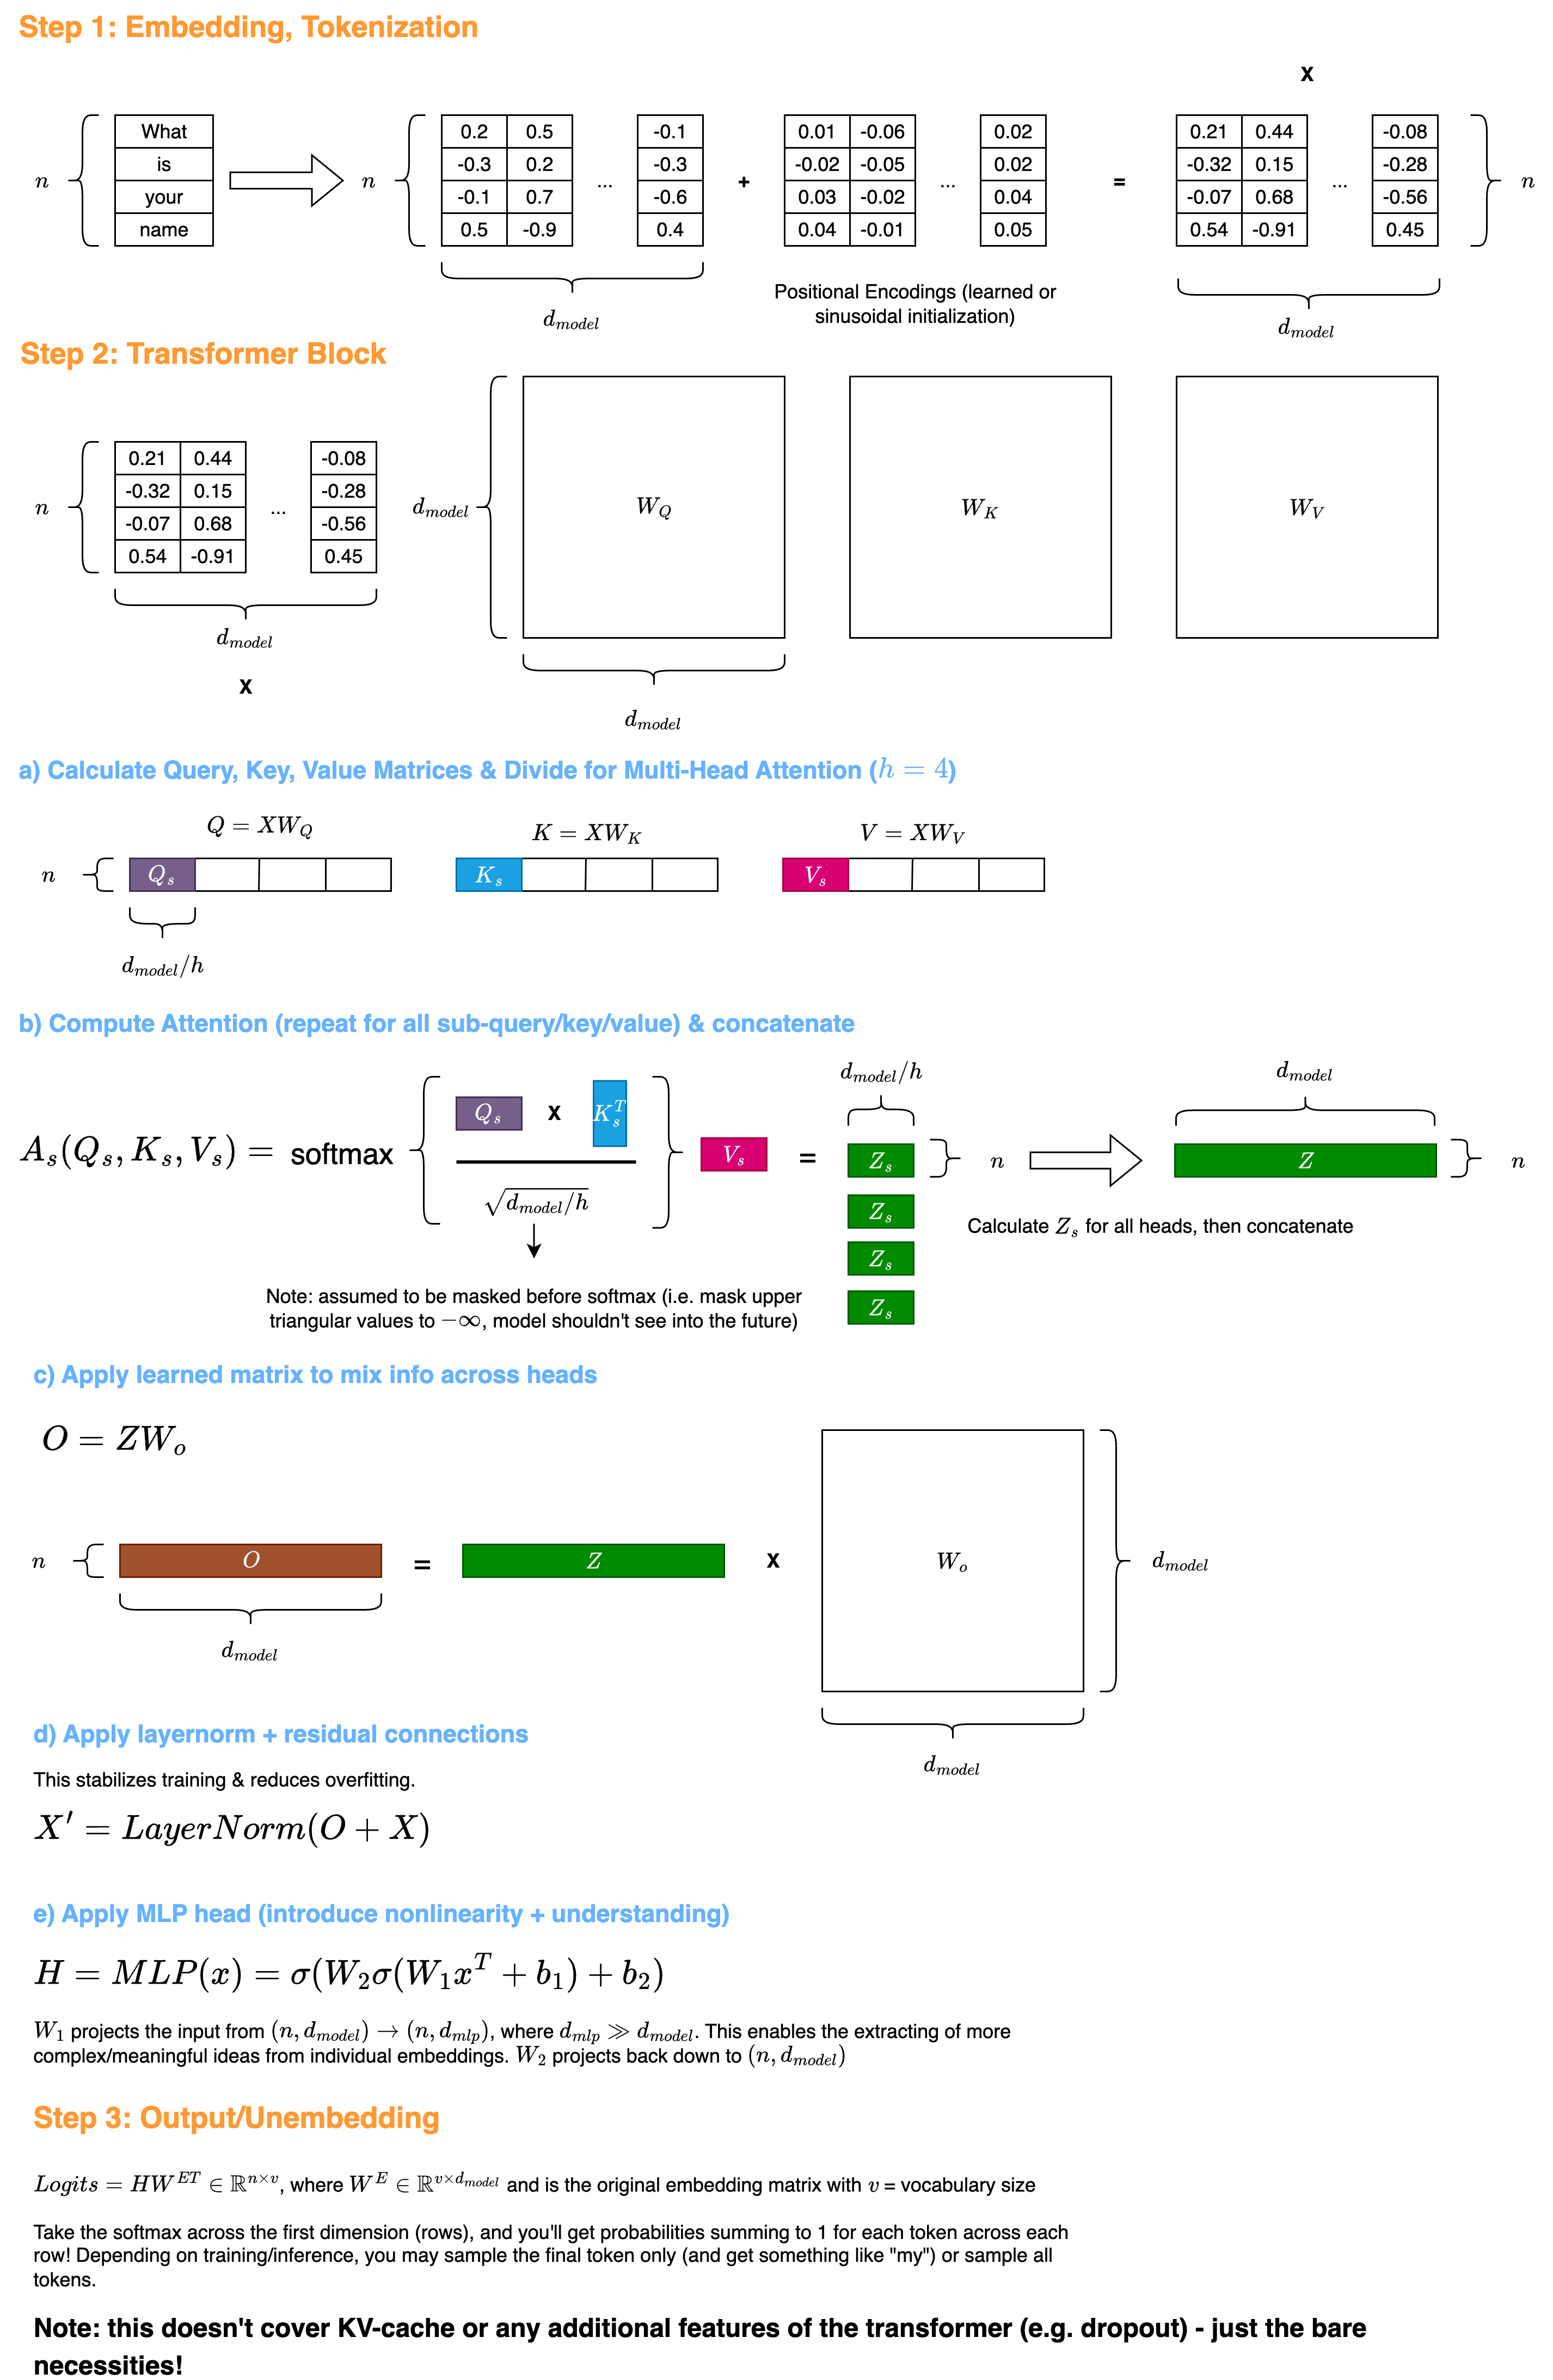
\includegraphics[width=0.8\textwidth]{../media/transformer.png}
    \caption{Transformer overview. Figure made by author. Zoom in to read better!}
    \label{fig:transformer}
\end{figure}

\subsection{Overview}

Transformers are composed of three parts:
\begin{enumerate}
  \item Encoding
  \item Transformer Blocks (Multi-Head Attention + MLP)
  \item Output
\end{enumerate}

Thinking about this from a high-level overview, in the case of a model like GPT, what might happen is as follows. Take some sentence composed of n words and embed those words using some algorithm into a higher dimensional space (n x $d_{model}$). Say that GPT has a vocabulary size of $v$. This embedding algorithm basically maps a token within that vocabulary to a new vector in $\mathbb{R}^{d_{model}}$.

The goal for each attention layer is to essentially "reweight" each of the $n$ embeddings based on information from other embeddings. At the end of the algorithm, the "reweighted" embeddings get "unembedded". The goal is to get a probability distribution over all possible tokens in the vocabulary for the next token after the current embedding. That can be done by taking the softmax over all the tokens in the vocabulary corresponding to each embedding. 

Here is where the training/inference procedure differs. If it's training, calculate the cross-entropy loss between the ground truth next token and the predicted token for EVERY word in the sentence. If it's inference, just extract the most probable next token from the LAST word in the sentence. 

Notably, some transformer models have encoders AND decoders, whereas others are only encoders (e.g. BERT) and others are only decoders (e.g. GPT). They differ in use cases, namely that encoder-based models are good for capturing deep semantic information whereas decoder-based models can generate new, realistic output. However, the difference between encoder-only and decoder-only models has been blurring a bit as models from both sides improve their understanding and generation capabilities. 

\subsection{Embedding}
Coming soon!
\subsection{Transformer Block}
Coming soon!
\subsection{Output}
Coming soon!
\subsection{Resources}
\begin{itemize}
  \item \href{https://arxiv.org/pdf/1706.03762}{Attention Is All You Need (Transformer paper)}
  
  \item \href{https://github.com/hyunwoongko/transformer}{PyTorch transformer implementation}
\end{itemize}

\section{Training Models}

\subsection{LMs: Reinforcement Learning with Human Feedback (RLHF)}

\begin{figure}[H]
    \centering
    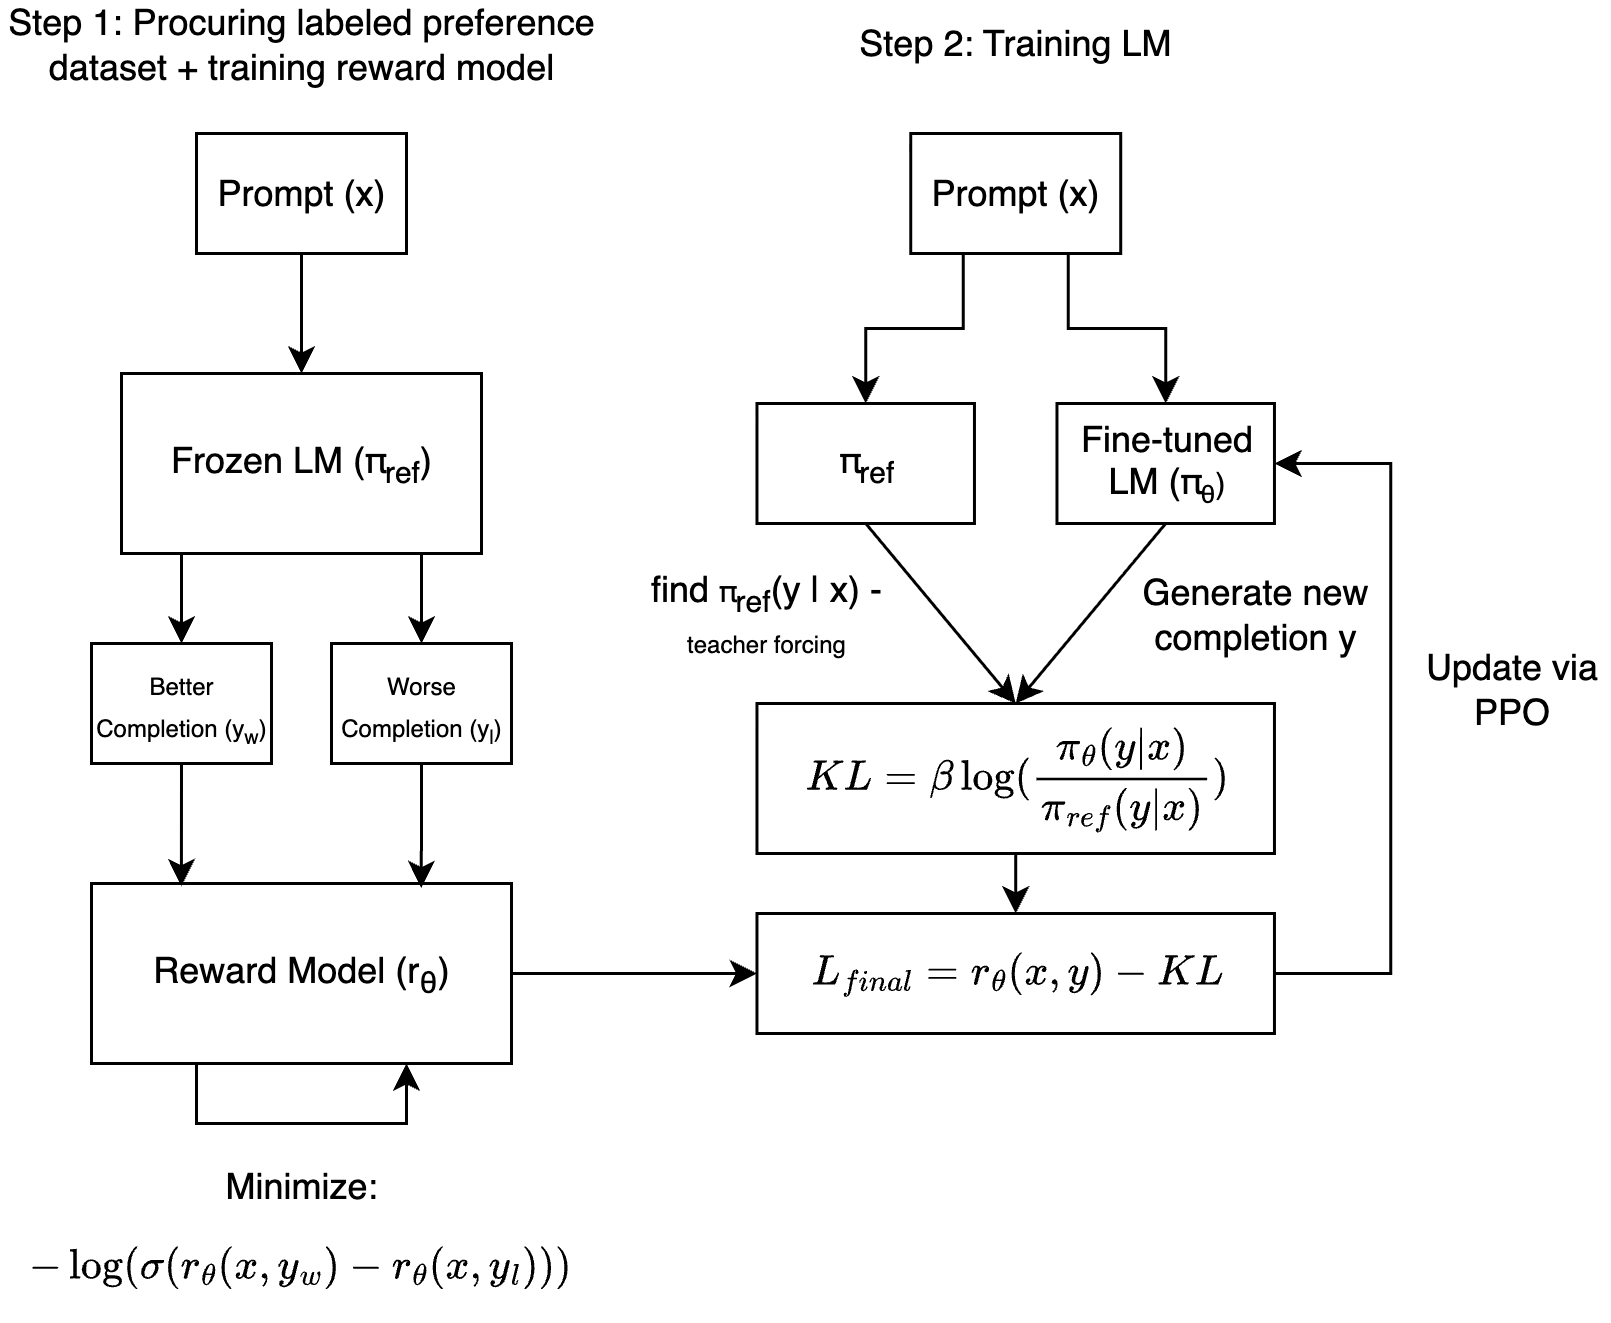
\includegraphics[width=1\textwidth]{../media/rlhf_light.png}
    \caption{RLHF overview. Figure made by author.}
    \label{fig:rlhf}
\end{figure}

Given some language model (LM) that's been pretrained on a large corpus of data (e.g. internet), we don't know how \textbf{reliable} or \textbf{aligned} that data is with human values. Thus, we want to \textbf{guide} the LM to incorporate basic human values, such as honesty, harmlessness, etc. Here's a high level overview of the process:

\begin{enumerate}
    \item \textbf{Reward Model}: procure a dataset of good/bad LM outputs relative to a prompt (via human annotators), train a reward model to maximize the difference in reward between good/bad prompt. Freeze the reward model after training. 
    \item \textbf{KL Divergence Calculation}: for any given prompt, calculate the KL divergence between frozen and unfrozen version of LM and subtract from the reward model output. 
    \item \textbf{PPO gradient update}: update weights of the unfrozen LM, and repeat step 2 and 3 until satisfactory performance is achieved. 
\end{enumerate}

\subsubsection{Reward Model}
We want to first train a reward model that models human preference. Given a pretrained reference model $\pi_{\mathrm{ref}}$, for each prompt $x^{(i)}$ where $i = 1, \ldots, N$, generate two outputs $y_w^{(i)}$ and $y_l^{(i)}$ such that:
\[
y_w^{(i)}, y_l^{(i)} \sim \pi_{\mathrm{ref}}(\cdot \mid x^{(i)})
\]
where $y_w^{(i)}$ is the preferred (higher-quality) completion and $y_l^{(i)}$ is the less preferred (lower-quality) completion for prompt $x^{(i)}$. This yields a dataset of $(y_w^{(i)}, y_l^{(i)}, x^{(i)})_{i=1}^{N}$. 

Next, use a reward model $r_{\phi}$ (perhaps just a transformer an added linear layer at the end) to process each sample in the dataset, minimizing the loss 

\[L_{reward} = -\logp{\sigp{r_{\phi}(y_w) - r_{\phi}(y_l)}}\]. This encourages the maximization of the reward for the good response while minimizing the reward for the bad response. 

\subsubsection{KL Divergence Calculation}
Now, we have a trained reward model. Let's freeze the weights of the original LM ($\pi_{ref}$) make a trainable copy of the original LM and call it $\pi_{\phi}$ (this will be the final fine-tuned LM after the entire process is complete). 

We need to prevent $\pi_{\phi}$ from "reward hacking" (i.e. giving nonsensical outputs to fool the reward model), so we calculate KL divergence between outputs of $\pi_{\phi}$ and $\pi_{ref}$. This is given as $KL = \beta\logp{\frac{\pi_{\phi}(y|x)}{\pi_{ref}(y|x)}}$. 

\subsection{LMs: Direct Preference Optimization (DPO)}
\begin{figure}[H]
    \centering
    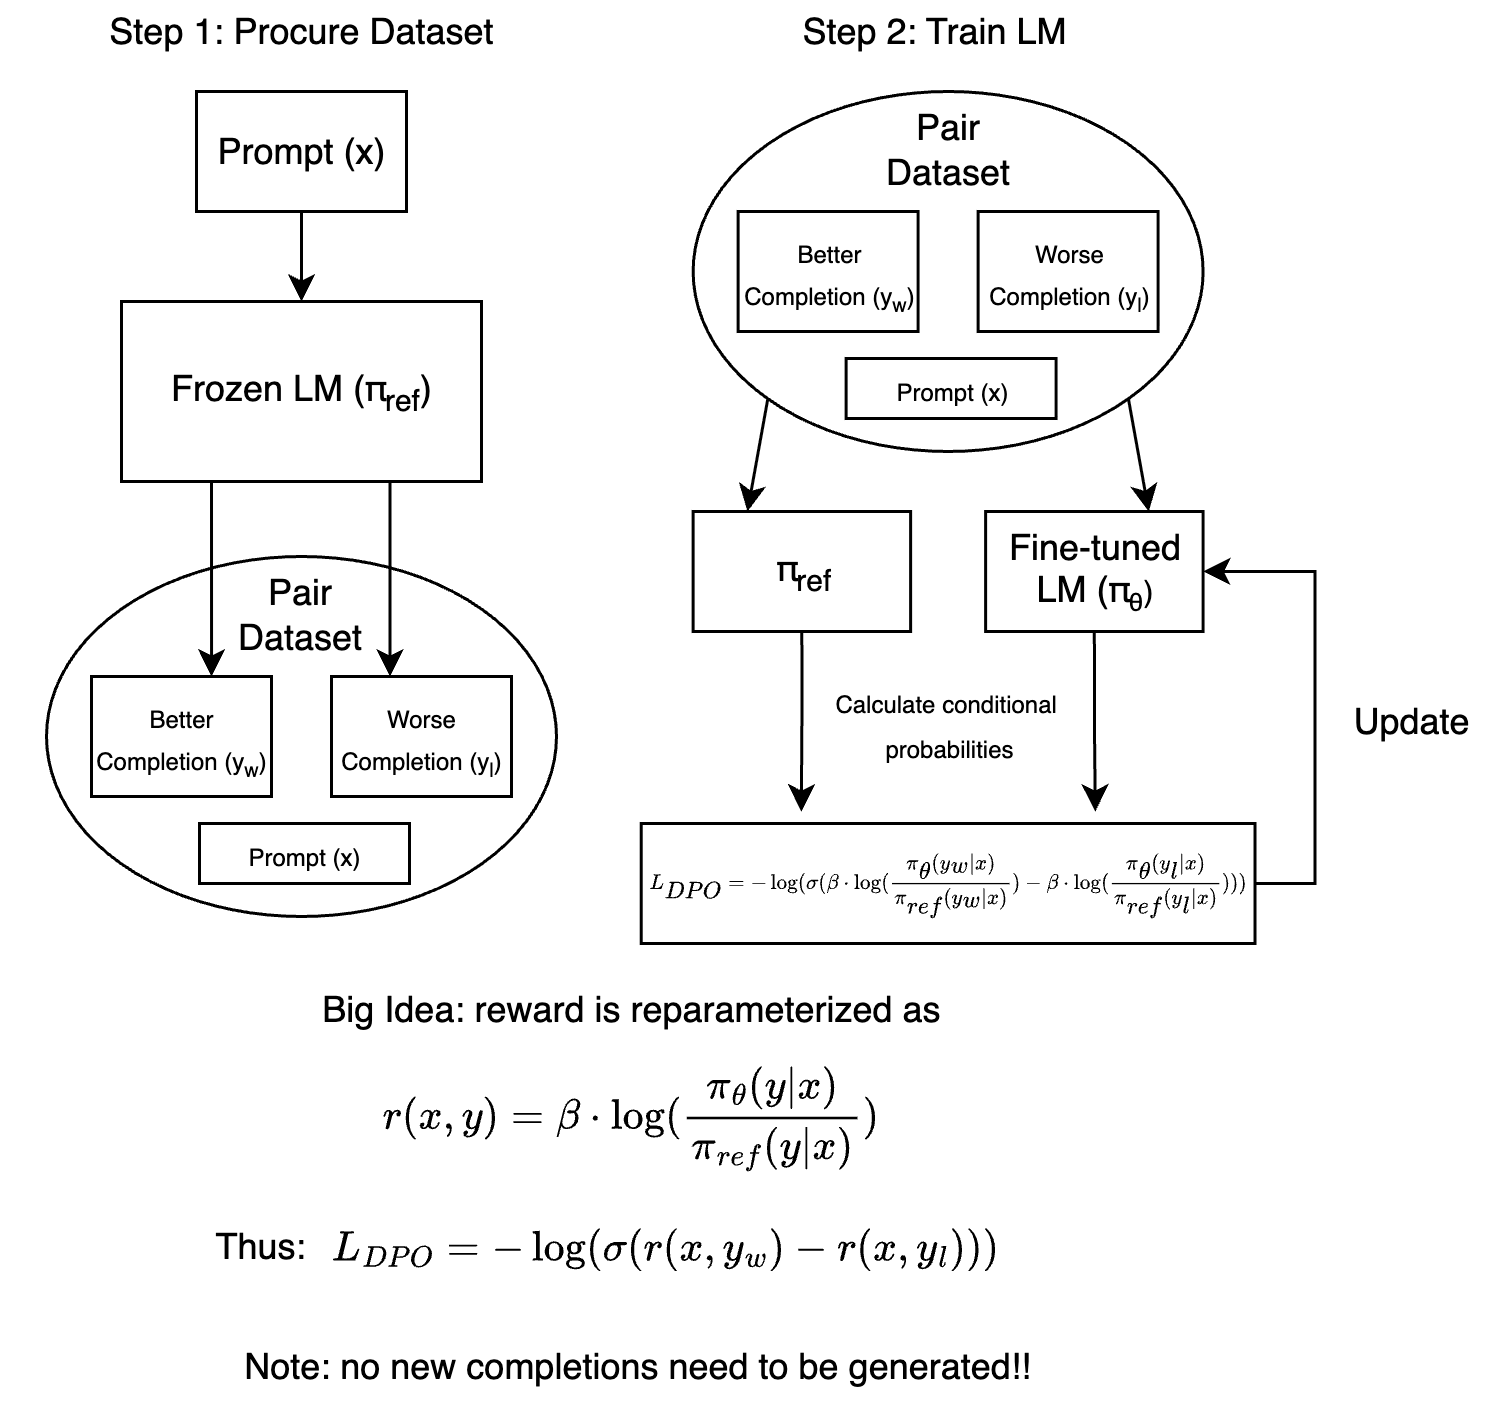
\includegraphics[width=0.8\textwidth]{../media/dpo_light.png}
    \caption{DPO overview. Figure made by author. }
    \label{fig:dpo}
\end{figure}

DPO eliminates the need for training an explicit reward model. The loss is formatted as $L_{DPO} = \log(\sigma(r_{\theta}(x, y_w) - r_{\theta}(x, y_l)))$. The goal is to reparameterize the reward function $r_{\theta}$ such that it's in terms of the original LM outputs (thus removing the need to train a separate reward model). Specifically, $r_{\theta}(x,y)$ is reparameterized as $
\beta \log(\frac{\pi_{\theta}(y | x)}{\pi_{ref}(y | x)}) + \beta Z(x)$. Briefly, $Z(x)$ is a partition function that represents some normalization factor over all possible outputs for the LM. For more information on the mathematical justification and details, visit the paper. Because we take the difference between $r_{\theta}(x, y_w)$ and $r_{\theta}(x, y_l)$, the $Z(x)$ term cancels out, which saves us a lot of time! Thus, the final loss is represented as:
\[
L_{DPO}=-\log(\sigma(\beta \cdot \log(\frac{\pi_{\theta}(y_w | x)}{\pi_{ref}(y_w | x)}) + \beta \cdot \log(\frac{\pi_{\theta}(y_l | x)}{\pi_{ref}(y_l | x)})))
\]

The authors argue that the intuition for why this approach works so well is because LMs can natively encode reward (hence "your language model is secretly a reward model"). Notably, DPO relies assumes the validity of the Bradley-Terry model. This states that human preference can be modeled by scalar values and pairwise comparisons are valid methods of determining the best model output. In reality, human preference is often not transitive (i.e. preferring A over B and preferring B over C does not always guarantee A is better than C). This is also a fundamental limitation for the normal RLHF setup. 

\subsection{Resources}
\begin{itemize}
    \item \href{https://arxiv.org/pdf/2203.02155}{Training language models to follow instructions with human feedback (RLHF paper)}

    \item \href{https://arxiv.org/pdf/2305.18290}{Direct Preference Optimization: Your Language Model is Secretly a Reward Model}
\end{itemize}

\end{document}